% easychair.tex,v 3.5 2017/03/15

\documentclass{easychair}
%\documentclass[EPiC]{easychair}
%\documentclass[EPiCempty]{easychair}
%\documentclass[debug]{easychair}
%\documentclass[verbose]{easychair}
%\documentclass[notimes]{easychair}
%\documentclass[withtimes]{easychair}
%\documentclass[a4paper]{easychair}
%\documentclass[letterpaper]{easychair}

\usepackage{doc}
\usepackage{tikz}
\usepackage{tikzsymbols}
\newtheorem{theorem}{Theorem}
\usetikzlibrary{arrows}

%\usepackage[firstpageonly=false, color={[gray]{0.5}},
%   scale=2.0, text=DRAFT]{draftwatermark}
% -------------------------------
%%%% For Alectryon

\usepackage{texments}
%%% for movies by alectryon
\usepackage{../movies/snippets/assets/alectryon}
\usepackage{../movies/snippets/assets/pygments}
%%% One hypothesis per line 
\makeatletter
\renewcommand{\alectryon@hyps@sep}{\alectryon@nl}
\makeatother

%%% \snippets{A,B,C,…} inputs a series of snippets as one block (with \itemsep
%%% between them).  A, B, C should be paths to files in movies/snippets/.
\usepackage{etoolbox}
\makeatletter
\newcommand{\inputsnippets}[1]
  {{\setlength{\itemsep}{1pt}\setlength{\parsep}{0pt}% Adjust spacing
    \alectryon@copymacros\begin{io}
      \forcsvlist{\item\@inputsnippet}{#1}
    \end{io}}}
\let\input@old\input % Save definition of \input
\newcommand{\@inputsnippet}[1]
  {{\renewenvironment{alectryon}{}{}% Skip \begin{alectryon} included in snippet
    \input@old{#1}}}
\makeatother

%---------------------------- 
\newcommand{\canonseq}[2]{\mbox{$\{#1\}(#2)$}}

\usepackage{varioref}
\newtheorem{todo}{To do}
\usepackage{amsfonts, afterpage}

\newcommand{\easychair}{\textsf{easychair}}
\newcommand{\miktex}{MiK{\TeX}}
\newcommand{\texniccenter}{{\TeX}nicCenter}
\newcommand{\makefile}{\texttt{Makefile}}
\newcommand{\latexeditor}{LEd}


%\makeindex

%% Front Matter
%%
% Regular title as in the article class.
%
\title{Hydras and Cie  \\
  Variations on Kirby \& Paris' hydra battles and ordinal numbers in Coq}



\author{
Pierre Castéran \inst{1}
\and
    Jérémy Damour \inst{2}
\and
Karl Palmskog \inst{3}
\and Clément Pit-Claudel \inst{4}
\and Théo Zimmermann \inst{5}
}


\institute{
Univ. Bordeaux, CNRS, Bordeaux INP, LaBRI, UMR 5800, F-33400 Talence, France \\
  \email{pierre.casteran@labri.fr}
\and
to fill!
\and
to fill!
\and
to fill!
\and
to fill!
 }



\authorrunning{Castéran, Damour, Palmskog, Pit-Claudel and Zimmermann}

\titlerunning{Hydras and Cie}

\begin{document}

\maketitle


\begin{abstract}
  \emph{Hydra-battles} is a collaborative library of commented proofs, developped under the \emph{Coq-Community} project.
  We present its evolution since a former presentation~\cite{JFLA2018paper} and how its structure is determined by other
  libraries and the \emph{Alectryon} literate proving tool.
\end{abstract}


% \setcounter{tocdepth}{2}
% {\small
% \tableofcontents}


%------------------------------------------------------------------------------
\section{Introduction}
\label{sect:introduction}
The \emph{Hydra-battles} project, part of \emph{Coq-Community}~\cite{CoqCommunity}  aims to be an experimental platform for the collaborative development of commented libraries of formal proofs. 


Hydra games (also known as \emph{Hydra battles}) appear in an article published in 1982 by two mathematicians, 
Laurie Kirby and Jeff Paris: \emph{Accessible Independence Results for Peano Arithmetic}~\cite{KP82}.
This article describes a game between two players: Hercules and a hydra.
A short description of the game  can be found in~\cite{bauer2008, KP82, JFLA2018paper}. One can also play with
Andrej Bauer's simulator~\cite{BauerHydra}.
In a few words:
\begin{itemize}
\item A hydra is a finite tree, traditionally presented with the root at the bottom, the leaves of which are called \emph{heads}
  (Fig~\ref{fig:round}).
\item At every round, Hercules chops off one head of the hydra. If the head is at a distance greater or equal than 2 from the root,
  then some sub-tree $h$ of the hydra is copied a certain amount $n$ of times. The number $n$ of copies and the sub-tree $h$ may depend of the considered variant of the game
  or the time elapsed since the beginning of the fight.
  Figure~\ref{fig:round} shows an example with $n=2$.
\end{itemize}



\begin{figure}[h]
  \centering
  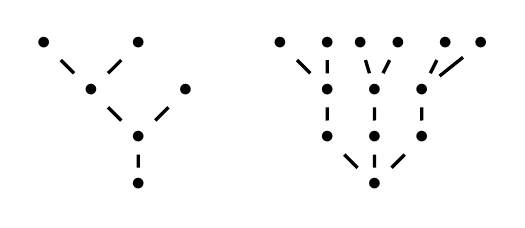
\begin{tikzpicture}[very thick, scale=0.3]
  \node (h1) at (4,0){$\bullet$};
  \node (h2) at (4,2){$\bullet$};
  \node (h3) at (2,4){$\bullet$};
  \node (h4) at (0,6){$\bullet$};
  \node (h5) at (4,6){$\bullet$};
  \node (h6) at (6,4){$\bullet$};
  \draw (h1) -- (h2) ;
  \draw (h2) -- (h3) ;
  \draw (h2) -- (h6);
  \draw (h3) -- (h4) ;
  \draw (h3) -- (h5) ;
 
\node (hn1) at (14,0){$\bullet$};
\node (hn2) at (12,2) {$\bullet$};
\node (hn3) at (12,4) {$\bullet$};
\node (hn4) at (10,6){$\bullet$};
  \node (hn5) at (12,6){$\bullet$};
  \draw (hn1) -- (hn2) ;
  \draw (hn2) -- (hn3) ;
  \draw (hn3) -- (hn4) ;
  \draw (hn3) -- (hn5) ;
\node (hn2b) at (14,2) {$\bullet$};
\node (hn3b) at (14,4) {$\bullet$};
\node (hn4b) at (13.4,6){$\bullet$};
  \node (hn5b) at (15,6){$\bullet$};
  \draw (hn1) -- (hn2b) ;
  \draw (hn2b) -- (hn3b) ;
  \draw (hn3b) -- (hn4b) ;
  \draw (hn3b) -- (hn5b) ;
  \node (hn2c) at (16,2) {$\bullet$};
\node (hn3c) at (16,4) {$\bullet$};
\node (hn4c) at (17,6){$\bullet$};
  \node (hn5c) at (18.5,6){$\bullet$};
  \draw (hn1) -- (hn2c) ;
  \draw (hn2c) -- (hn3c) ;
  \draw (hn3c) -- (hn4c) ;
  \draw (hn3c) -- (hn5c) ;
\end{tikzpicture}

  \caption{Two successive states of a hydra in a battle}
  \label{fig:round}
\end{figure}


 %  \begin{figure}[htb]
% \centering
% \begin{tikzpicture}[very thick, scale=0.3]
% \node (foot) at (10,0) {$\bullet$};
% \node (N1) at (2,2) {$\bullet$};
% \node (N2) at (10,2) {$\bullet$};
% \node (N22) at (7,2) {$\bullet$};
% \node (N3) at (14,2) {$\bullet$};
% \node (N4) at (18,2) {$\Smiley[2][green]$};
% \node (N5) at (0,4) {$\bullet$};
% \node (N6) at (2,5) {$\Smiley[2][green]$};
% \node (N7) at (4,6) {$\Smiley[2][green]$};
% \node (N88) at (7,4) {$\bullet$};
% \node (N8) at (10,4) {$\bullet$};
% \node (N9) at (14,6) {$\Smiley[2][green]$};
% \node (N10) at (0,8) {$\Smiley[2][green]$};
% \node (N11) at (10,7) {$\Smiley[2][green]$};
% \node (N111) at (7,7) {$\Smiley[2][green]$};
% \draw (foot) to [bend left=10] (N1);
% \draw (foot) -- (N2);
% \draw (foot) -- (N22);
% \draw (foot) -- (N3);
% \draw (foot) -- (N4);
% \draw (N1) to  (N5);
% \draw (N1) to   [bend left=10] (N6);
% \draw (N1) to   [bend right=20] (N7);
% \draw (N2) to  (N8);
% \draw (N22) to  (N88);
% \draw (N8) to  (N11);
% \draw (N88) to  (N111);
% \draw (N3) to  (N9);
% \draw (N5) to  (N10);
% \end{tikzpicture}
% \caption{The hydra associated with the ordinal $\omega^{\omega+2}+\omega^\omega \times 2 + \omega + 1$ \label{fig:iota-example}}

% \end{figure}

Kirby and Paris prove the following theorems, applying
combinatorial results about ordinal numbers by Jussi Ketonen and Robert Solovay~\cite{KS81}.

\begin{theorem}
  In the Hydra game, every strategy is a winning strategy for Hercules. \label{kp:thm1}
\end{theorem}

\begin{theorem}
  Theorem~\ref{kp:thm1} cannot be proved in Peano Arithmetic. \label{kp:thm2}
\end{theorem}

The contrast between the simplicity of the statements above and the complexity of their proofs convinced us that it is a good thema for a commented library~\cite{HydraBattles} of formal proofs written for the \textit{Coq} proof assistant~\cite{Coq}. 

Complex formalisations and proofs are explained in an
  electronic book~\cite{HydraBook}. Whenever various reasonable choices exist, we try to present and compare the alternatives.
  For instance, Figures~\ref{fig:Ex42E0} and \ref{fig:Ex42-schutte} show two radically different proofs of the equality
  $\omega+42+\omega^2=\omega^2$, the first one is a simple proof by computation, the second one shows how this equality
  is a consequence of the axioms of the set-theoretic model  by Kurt Schütte~\cite{schutte}. 

This work is also an opportunity to 
 provide ``concrete'' examples of formalization and proof techniques: operational type classes, functions defined by  equations, dependently typed functions, etc. It may be also used as a library on ordinal numbers, for instance for proving termination properties.

 Prior stages of this project have already been presented at
 JFLA~\cite{PCiota, JFLA2018paper}.
We present the recent evolutions of the library: new results, interaction within the Coq-Community project~\cite{CoqCommunity}, and documentation generated with Alectryon~\cite{alectryonpaper, alectryongithub}.

\section{Changes in the library}
The 2018 article~\cite{JFLA2018paper} contains a formal proof of  a variant of Theorem~\ref{kp:thm2}:

\begin{theorem}
  There is no termination measure mapping hydras to a segment $[0,\mu)$ where $\mu<\epsilon_0$ for proving the termination of  all hydra battles.\label{thm3}
\end{theorem}

Indeed, the consideration of \emph{all} battles allowed us to
consider battles where the hydra can make an arbitrary number of copies at any time, which made artificially easier our proof by absurd.
Unfortunately, the examples  most shown in the litterature
(see for instance \cite{KP82, bauer2008, BauerHydra}) 
assume that the hydra grows $n$ copies at step $n$ of the game, which is incompatible with our proof.

\vspace{6pt}

We prove now that Theorem~\ref{thm3} still holds with this ``usual'' kind of battles, by borrowing new combinatorial results from~\cite{KS81}.
Without loss of generality, we could consider the following restrictions:
 
 \begin{itemize}
   \item The game starts at an initial step $i\in\mathbb{N}$ (not necessarily $0$).
   \item  The hydra is always the the graphical representation of some ordinal strictly below $\epsilon_0$ in Cantor normal
     form. For instance, Fig~\ref{fig:round} shows the hydras respectively associated with  $\omega^{\omega^2+1}$ and $\omega^{\omega^2}\times 3$.
 
 \item Hercules always chops off the rightmost head of the hydra.
 \end{itemize}
 
 It mathematical terms, if at step $n$ the hydra is associated with the ordinal $\alpha$, at step $n+1$ it is associated with
 $\canonseq{\alpha}{n+1}$, the $(n+1)$th element of the canonical sequence of $\alpha$~\cite{KS81}.
 
 
Let $\alpha<\epsilon_0$ be an ordinal.
Using the \texttt{coq-equations} plug-in~\cite{sozeau:hal-01671777}, we define the function which returns the number of steps of the battle starting with $\alpha$ at step $i$ for  any $i\in\mathbb{N}$.
We prove that this number is greater or equal than
$H'_\alpha(i)-i$, where $H'$ is a slight variant of the Wainer Hardy hierarchy of rapidly growing functions~\cite{BW85, KS81, Promel2013, Wainer1970}, defined by transfinite recursion in Fig.~\ref{fig:Hprime}.
From this result, we infer that the considered function is not primitive recursive in general (for $\alpha\geq\omega^\omega$).

\begin{figure}[h]
  \centering
  \begin{itemize}
\item If $\alpha=0$, then $H'_\alpha (i)= i$ for any natural number $i$.
\item If $\alpha=\beta+1$, then 
$H'_\alpha(i)=H'_\beta(i+1)$ for any $i \in \mathbb{N}$.
\item If $\alpha$ is a limit ordinal, then 
$H'_\alpha(i) = H'_{(\canonseq{\alpha}{i+1})}(k)$ for any $i\in \mathbb{N}$.
\end{itemize}
\vspace{4pt}
\inputsnippets{HprimeDef}
\caption{The rapidly growing hierarchy $H'$ of arithmetic functions}
\label{fig:Hprime}
\end{figure}

\label{sect:not-pr}



 
\section{Main features}




\subsection{The Coq-Community ecosystem}
\begin{todo}
Small presentation.
\end{todo}

In order to prove formally that the length of the considered
kind of battles is not given by a primitive recursive function, weused the formalization of primitive recursive functions, part
of Russell O'Connor's contribution on G\"{o}del first incompleteness theorem \cite{OConnor05, Goedel}.
For this purpose, and above all by consideration of the scientific interest of this contribution, we chose to host and maintain this work within \textit{Coq-Community}.

Computability is a key topic in Computer Science teaching. Moreover O'Conor's library is a nice illustration of dependently typed programming, so we chose to devote a full chapter to this formalisation, with comments on the definitions and proofs, [counter]-examples and exercises.


\subsection{Documentation with Alectryon}
\begin{todo}
  Interest of Alectryon:
  \begin{itemize}
  \item Despite the frequent changes (improvements) in the Coq scripts, code inclusion and \textit{Coq}'s answers are up to date.

  \item Presentation of the main steps of proofs, possibly interleaved with text.
      
  \end{itemize}

   Figures~\ref{fig:Hprime} (code snippet), \ref{fig:Ex42E0} and \ref{fig:Ex42-schutte} have been generated with Alectryon.
\end{todo}


  \begin{figure}[h]
    \centering
    \fbox{
      \begin{minipage}[h]{1.0\linewidth}
        \inputsnippets{Ex42}
      \end{minipage}}
    \caption{A simple proof by computation}
    \label{fig:Ex42E0}
  \end{figure}



%\afterpage{\clearpage}

\begin{figure}[th]
  \centering
  
  

\fbox{\begin{minipage}[h]{1.0\linewidth}
  Let us prove again the equality $\omega+42+\omega^2= \omega^2$. Let us recall that $\omega^2$ is an abbreviation of $\phi_0(2)$,
\emph{i.e} the third  additive principal ordinal.

\inputsnippets{Ex42a}


Our proof is very different from the computational proof of Fig\ref{fig:Ex42E0}.
By definition of additive principal ordinals, 
it suffices to prove the inequality $\omega+42< \phi_0(2)$.

\inputsnippets{Ex42b}

Since the set \textit{AP} of additive principals  is closed under addition
(by Lemma \textit{AP\_plus\_closed}), it suffices to prove the inequalities $\omega<\phi_0(2)$ and $42<\phi_0(2)$.

\inputsnippets{Ex42d, Ex42c, Ex42e}

\end{minipage}
}
\caption{A proof interleaved with text (from the book)}
  \label{fig:Ex42-schutte}
\end{figure}

\section{Conclusion and perspectives}




%\subsection{Perspectives}


The Gaia project~\cite{Gaia}, also maintained on \textit{Coq-Community} contains a development by José Grimm~\cite{grimm:hal-00911710}. This library -- dedicated  to the implementation in \textit{Coq (SSreflect)} of books from  Bourbaki's Elements of Mathematics --- contains a generalization of two types of ordinals (\texttt{T1} for the ordinal $\epsilon_0$ and
\texttt{T2} for $\Gamma_0$) to a larger ordinal defined by Ackermann, and relates these data structures with Bourbaki's set theory.
It is interesting to note that both libraries \textit{Gaia} and \textit{hydra-battles} contain their own (isomorphic but not identical) definitions of types \texttt{T1} and \texttt{T2}, both originated in~\cite{CantorContrib}.
Our plan is to build a  ``gate'' giving access to both the combinatorial results of \textit{hydra-battles} and the set-theoretic content of \textit{Gaia}, and make possible the transfer of theorems from one of the two libraries to the other one.

Another direction would be to write in \textit{Coq} a formal proof of the original statement of Theorem~\ref{kp:thm2}. For this purpose, we plan to import  the formalization of Peano Arithmetic by O'Connor~\cite{Goedel}.

 \emph{Hydra-battles} is not limited to the study of ordinal numbers and applications.
 For instance, we are also developing 
a module about efficient exponentiation algorithms, and hope
to extend our project to new topics.

%\section{Acknowledgments}
%\label{sect:acks}



\label{sect:bib}
\bibliographystyle{plain}
%\bibliographystyle{alpha}
%\bibliographystyle{unsrt}
%\bibliographystyle{abbrv}
\bibliography{../thebib}


\end{document}

